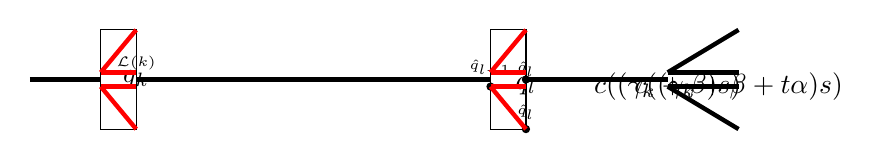
\begin{tikzpicture}[scale=0.9]
    \draw[ultra thick] (-3,0)--(6,0);
    \draw[fill=white] (-2,-0.1)--(-1.5,-0.1)--(-1.5,-0.7)--(-2,-0.7)--cycle;
    \draw[fill=white] (-2,-0.1)--(-1.5,-0.1)--(-1.5,0.7)--(-2,0.7)--cycle;
    \node at (-1.5,0) {$q_k$};
    \node[above] at (-1.5,0) {\tiny$\mathcal{L}(k)$};
    \draw[red, ultra thick] (-2,-0.1)--(-1.5,-0.1);
    \draw[red, ultra thick] (-2,-0.1)--(-1.5,-0.7);
    \draw[red, ultra thick] (-2,0.1)--(-1.5,0.1);
    \draw[red, ultra thick] (-2,0.1)--(-1.5,0.7);
    \draw[ultra thick] (2.5,0)--(4,0);
    \draw[fill=white] (3.5,-0.1)--(4,-0.1)--(4,-0.7)--(3.5,-0.7)--cycle;
    \draw[fill=white] (3.5,-0.1)--(4,-0.1)--(4,0.7)--(3.5,0.7)--cycle;
    \node at (4,-0.1) {$q_l$};
    \draw[fill=black] (4,0) circle (.05cm);
    \draw[fill=black] (4,-0.7) circle (.05cm);
    \node[above] at (4,-0.1) {\tiny$\hat{q}_{l}$};
    \node[above] at (4,-0.7) {\tiny$\hat{q}_{l}$};
    \draw[fill=black] (3.5,-0.1) circle (.05cm);
    \node[above] at (3.5,-0.1) {\tiny$\hat{q}_{l-1}$};
    \draw[red, ultra thick] (3.5,-0.1)--(4,-0.1);
    \draw[red, ultra thick] (3.5,-0.1)--(4,-0.7);
    \draw[red, ultra thick] (3.5,0.1)--(4,0.1);
    \draw[red, ultra thick] (3.5,0.1)--(4,0.7);
    \draw[ultra thick] (6,-0.1)--(7,-0.1);
    \draw[ultra thick] (6,-0.1)--(7,-0.7);
    \draw[ultra thick] (6,0.1)--(7,0.1);
    \draw[ultra thick] (6,0.1)--(7,0.7);
    \node at (7,-0.1) {$c((\gamma_k+\beta+t\alpha)s)$};
    \node at (6,-0.1) {$c((\gamma_k+\beta)s)$};
    \end{tikzpicture}